\section{Experiments}
\label{sec:eval}

We assess \ours in two long-context domains: conversational agents and document analysis. For conversational agents, we expand the existing Multi-Session Chat dataset \cite{xu2021mscbeyond} and introduce two new dialogue tasks that evaluate an agent's ability to retain knowledge across long conversations. For document analysis, we benchmark \ours on existing tasks from \cite{liu2023lostinmiddle} for question answering and key-value retrieval over lengthy documents. We also propose a new nested key-value retrieval task requiring collating information across multiple data sources, which tests the ability of an agent to collate information from multiple data sources (multi-hop retrieval). We publicly release our augmented MSC dataset, nested KV retrieval dataset, and a dataset of embeddings for 20M Wikipedia articles to facilitate future research. Our code for the benchmarks is available at \website. 

\textbf{Implementation details.} When discussing OpenAI models, unless otherwise specified `GPT-4 Turbo' refers to the specific \texttt{gpt-4-1106-preview} model endpoint (context window of $128,000$), `GPT-4` refers to \texttt{gpt-4-0613} (context window of $8,192$), and `GPT-3.5 Turbo` refers to \texttt{gpt-3.5-turbo-1106} (context window of $16,385$). In experiments, we run \ours with all baseline models (GPT-4, GPT-4 Turbo, and GPT 3.5) to show how the underlying model performance affects \ours's. 






\subsection{\ours for conversational agents}

Conversational agents like virtual companions and personalized assistants aim to engage users in natural, long-term interactions, potentially spanning weeks, months, or even years. This creates challenges for models with fixed-length contexts, which can only reference a limited history of the conversation. An `infinite context' agent should seamlessly handle continuous exchanges without boundary or reset. When conversing with a user, such an agent must satisfy two key criteria:
(1) Consistency - The agent should maintain conversational coherence. New facts, preferences, and events mentioned should align with prior statements from both the user and agent.
(2) Engagement - The agent should draw on long-term knowledge about the user to personalize responses. Referencing prior conversations makes dialogue more natural and engaging.

We therefore assess our proposed system, \ours, on these two criteria:
(1) Does \ours leverage its memory to improve conversation consistency? Can it remember relevant facts, preferences, and events from past interactions to maintain coherence?
(2) Does \ours produce more engaging dialogue by taking advantage of memory? Does it spontaneously incorporate long-range user information to personalize messages?
By evaluating on consistency and engagement, we can determine how well \ours handles the challenges of long-term conversational interaction compared to fixed-context baselines. Its ability to satisfy these criteria will demonstrate whether unbounded context provides meaningful benefits for conversational agents.







\begin{table}[t!]
\caption{
\textbf{Deep memory retrieval (DMR) performance.}
In this task, the agent is asked a specific question about a topic discussed in a prior conversation (sessions 1--5).
The agent's response is scored against the gold answer.
\ours significantly outperforms the fixed-context baselines.
}
\label{table:deep-memory-task}

\begin{center}
\begin{tabular}{lrr}
\toprule
\bf Model & \textbf{Accuracy} $\Uparrow$ & \bf ROUGE-L (R) $\Uparrow$ \\
\midrule

GPT-3.5 Turbo & 38.7\% & 0.394  \\
$+$ MemGPT & 66.9\% & 0.629 \\


GPT-4 & 32.1\% & 0.296 \\

$+$ MemGPT & 92.5\% & 0.814  \\


GPT-4 Turbo & 35.3\% & 0.359  \\

$+$ \textbf{MemGPT} & \textbf{93.4\%} & \textbf{0.827}  \\

\bottomrule
\end{tabular}
\end{center}

\end{table}


\textbf{Dataset.}
We evaluate \ours and our fixed-context baselines on the Multi-Session Chat (MSC) dataset introduced by \citet{xu2021mscbeyond}, which contains multi-session chat logs generated by human labelers, each of whom was asked to play a consistent persona for the duration of all sessions. Each multi-session chat in MSC has five total sessions, and each session consists of a roughly a dozen messages.
As part of our consistency experiments, we created a new session (session 6) that contains a single question-answer response pair between the same two personas. 



\subsubsection{Deep memory retrieval task (consistency).}
We introduce a new `deep memory retrieval' (DMR) task based on the MSC dataset designed to test the consistency of a conversational agent. In DMR, the conversational agent is asked a question by the user that explicitly refers back to a prior conversation and has a very narrow expected answer range. We generated the DMR question-answer (QA) pairs using a separate LLM that was instructed to write a question from one user to another that could only be answered correctly using knowledge gained from the past sessions (see Appendix for further details).

We evaluate the quality of the generated response against the `gold response' using ROUGE-L scores \citep{lin2004rouge} and an `LLM judge', which is instructed to evaluate whether or not the generated response is consistent with the gold response (GPT-4 has been shown to have high agreement with human evaluators \citep{zheng2023llmasajudge}).
In practice, we notice that the generated responses (from both \ours and the baselines) were generally more verbose than the gold responses.
We use the ROUGE-L recall (R) metric to account for the verbosity of the generated agent replies compared to the relatively short gold answer labels.









\begin{table}[t]
\caption{
\textbf{Conversation opener performance.}
The agent's conversation opener is evaluated using similarity scores to the gold persona labels (SIM-1/3) and to the human-created opener (SIM-H). 
MemGPT is able to exceed the performance of the human-created conversation opener with a variety of underlying models.
}
\label{table:msc-opener-task}
\begin{center}
\begin{tabular}{lrrr}
\toprule
\bf Method 
&  $\Uparrow$ \textbf{SIM-1} & \textbf{SIM-3} & \textbf{SIM-H}
\\
\midrule
Human & 0.800 & 0.800 & 1.000  \\
\midrule
GPT-3.5 Turbo & 0.830 & 0.812 & \bf 0.817 \\
GPT-4 &  \bf 0.868 &  \bf 0.843 &  0.773 \\
GPT-4 Turbo & 0.857 & 0.828 & 0.767 \\
\bottomrule
\end{tabular}
\end{center}
\end{table}


\textbf{\ours utilizes memory to maintain coherence:}
Table \ref{table:deep-memory-task} shows the performance of \ours vs the fixed-memory baselines.
We compare MemGPT using different underlying LLMs, and compare against using the base LLM without MemGPT as a baseline.
The baselines are able to see a lossy summarization of the past five conversations to mimic an extended recursive summarization procedure, while MemGPT instead has access to the full conversation history but must access it via paginated search queries to recall memory (in order to bring them into main context).
In this task, we see that MemGPT clearly improves the performance of the underlying base LLM: there is a clear drop in both accuracy and ROUGE scores when going from MemGPT to the corresponding LLM baselines.



\subsubsection{Conversation opener task (engagement).}
In the `conversation opener' task we evaluate an agent's ability to craft engaging messages to the user that draw from knowledge accumulated in prior conversations.
To evaluate the `engagingness' of a conversation opener using the MSC dataset, we compare the generated opener to the gold personas: an engaging conversation opener should draw from one (or several) of the data points contained in the persona, which in MSC effectively summarize the knowledge accumulated throughout all prior sessions.
We also compare to the human-generated gold opener, i.e., the first response in the following session.
We report the CSIM scores of \ours's openers in Table~\ref{table:msc-opener-task}.
We test several variations of \ours using different base LLMs.






\begin{figure}[t!]
\begin{center}
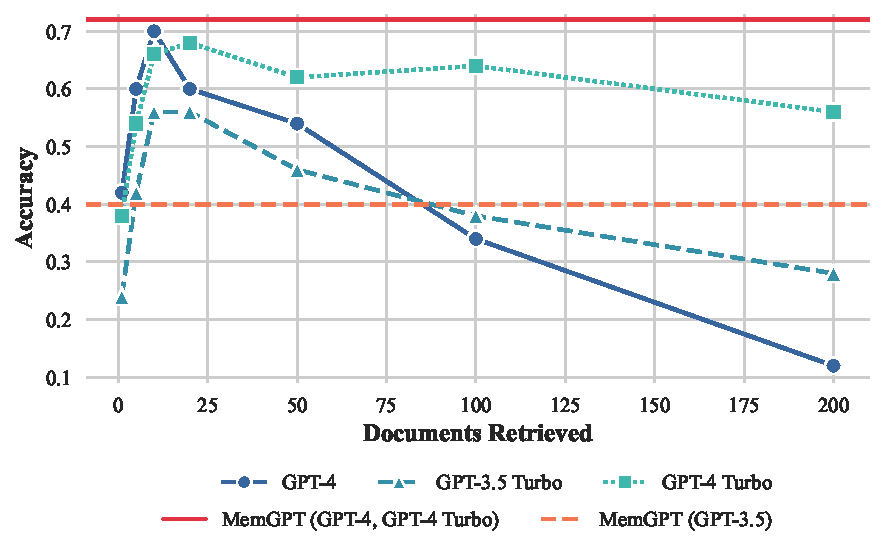
\includegraphics[width=0.48\textwidth]{images/docqa.pdf}
\end{center}
\caption{
\textbf{Document QA task performance.}
\ours's performance is unaffected by increased context length. Methods such as truncation can extend the effective context lengths of fixed length models such as GPT-4, but such compression methods will lead to performance degradation as the necessary compression grows. Running \ours with GPT-4 and GPT-4 Turbo have equivalent results on this task.
}
\label{fig:doc_qa_task_results}
\end{figure}



\textbf{\ours utilizes memory to increase engagement:}
As seen in Table~\ref{table:msc-opener-task}, \ours is able to craft engaging openers that perform similarly to and occasionally exceed the hand-written human openers. 
We observe that \ours tends to craft openers that are both more verbose and cover more aspects of the persona information than the human baseline.
Additionally, we can see the storing information in working context is key to generating engaging openers.









\subsection{\ours for document analysis}


Document analysis also faces challenges due to the limited context windows of today's transformer models. As shown in Table \ref{context-length-comparison}, both open and closed source models suffer from constrained context length (up to 128k tokens for OpenAI's models). However many documents easily surpass these lengths; for example, legal or financial documents such as Annual Reports (SEC Form 10-K) can easily pass the million token mark. Moreover, many real document analysis tasks require drawing connections across multiple such lengthy documents. Anticipating these scenarios, it becomes difficult to envision blindly scaling up context as a solution to the fixed-context problem. Recent research \citep{liu2023lostinmiddle} also raises doubts about the utility of simply scaling contexts, since they find uneven attention distributions in large context models (the model is more capable of recalling information at the beginning or end of its context window, vs tokens in the middle). To enable reasoning across documents, more flexible memory architectures like \ours are needed.

\begin{figure}[t!]
    \centering
\begin{center}
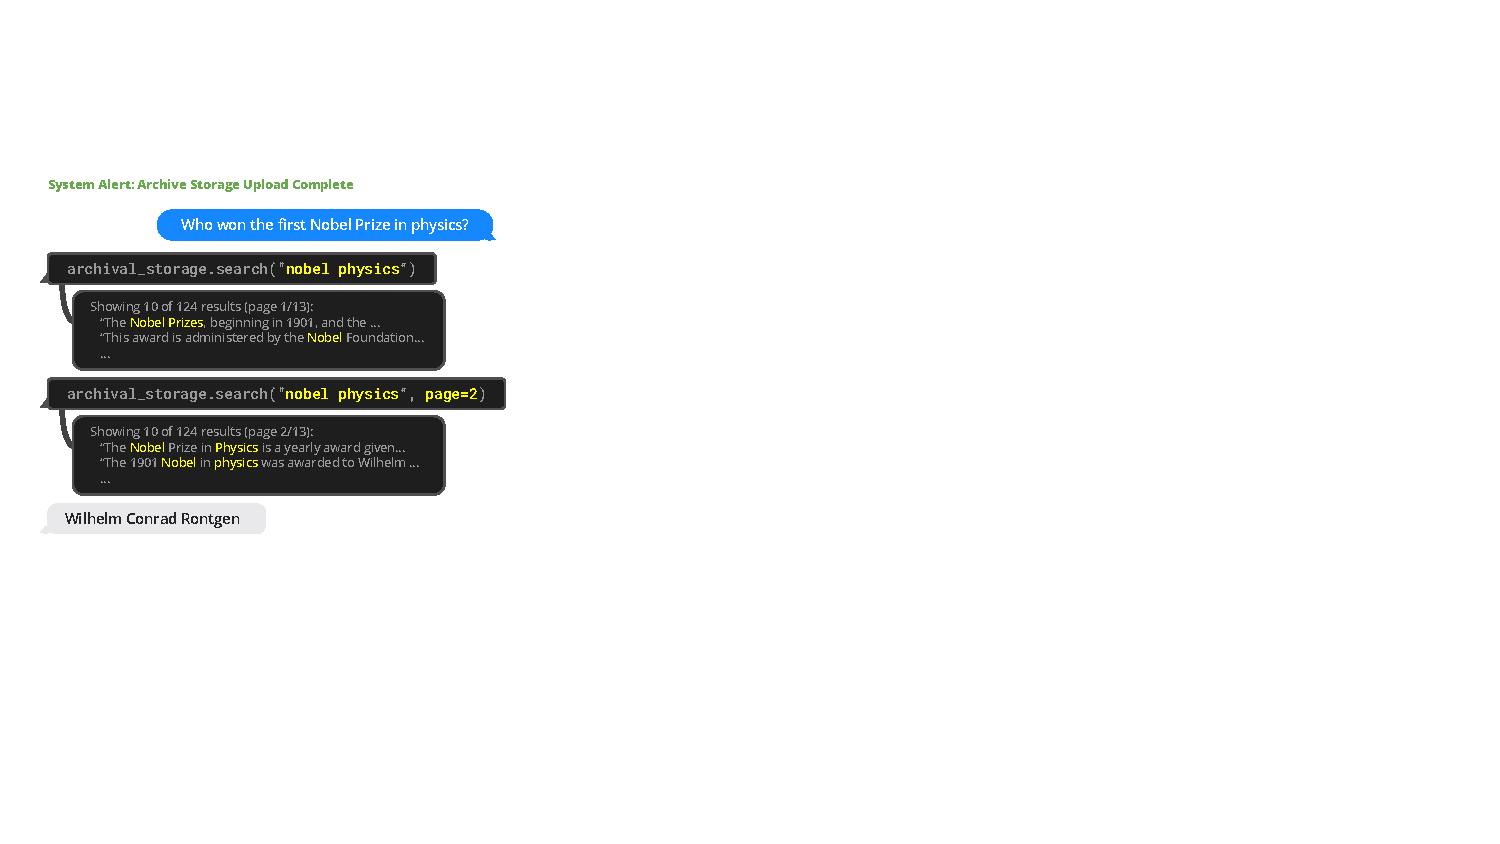
\includegraphics[width=0.45\textwidth]{images/memgpt_docqa_example_2.pdf}
\end{center}
    \caption{
An example of MemGPT (left) solving the document QA task. A database of Wikipedia documents is uploaded to archival storage.  MemGPT queries archival storage via function calling, which pulls paginated search results into main context.
}
    \label{fig:example-docqa}
\end{figure}








\subsubsection{Multi-document question-answering.} 
To evaluate \ours's ability to analyze documents, we benchmark \ours against fixed-context baselines on the retriever-reader document QA task from \citet{liu2023lostinmiddle}. 
In this task, a question is selected from the NaturalQuestions-Open dataset, and a retriever selects relevant Wikipedia documents for the question. A reader model (the LLM) is then fed these documents as input, and is asked to use the provided documents to answer the question. 
Similar to \citet{liu2023lostinmiddle}, 
we evaluate reader accuracy as the number of retrieved documents $K$ increases.

In our evaluation setup, both the fixed-context baselines and \ours use the same retriever, which selects the top $K$ documents according using similarity search (cosine distance) on OpenAI's \texttt{text-embedding-ada-002} embeddings. We use MemGPT's default storage settings which uses PostgreSQL for archival memory storage with vector search enabled via the pgvector extention. We pre-compute embeddings and load them into the database, which uses an HNSW index to enable approximate, sub-second query times. 
In \ours, the entire embedding document set is loaded into archival storage, and the retriever naturally emerges via the archival storage search functionality (which performs vector search based on cosine similarity). 
In the fixed-context baselines, the top-$K$ documents are fetched using the retriever independently from the LLM inference, similar to the original retriever-reader setup in \citet{liu2023lostinmiddle}. 

We use a dump of Wikipedia from late 2018, following past work on NaturalQuestions-Open \citep{izacard2020leveraging, izacard2021unsupervised}, and sampled a subset of 50 questions for evaluation. Both the sampled questions and embedded Wikipedia passages are publicaly released. We evaluate the performance of both \ours and baselines with an LLM-judge, to ensure that the the answer is properly derived from the retrieved documents and to avoid non-exact string matches being considered incorrect. 


We show the results for the document QA task in Figure \ref{fig:doc_qa_task_results}. The fixed-context baselines performance is capped roughly at the performance of the retriever, as they use the information that is presented in their context window (e.g. if the embedding search retriever fails to surface the gold article using the provided question, the fixed-context baselines are guaranteed to never see the gold article). 
By contrast, \ours is effectively able to make multiple calls to the retriever by querying archival storage, allowing it to scale to larger effective context lengths. 
\ours actively retrieves documents from its archival storage (and can iteratively page through results), so the total number of documents available to \ours is no longer limited by the number of documents that fit within the LLM processor's context window.

\begin{figure}[t!]
\begin{center}
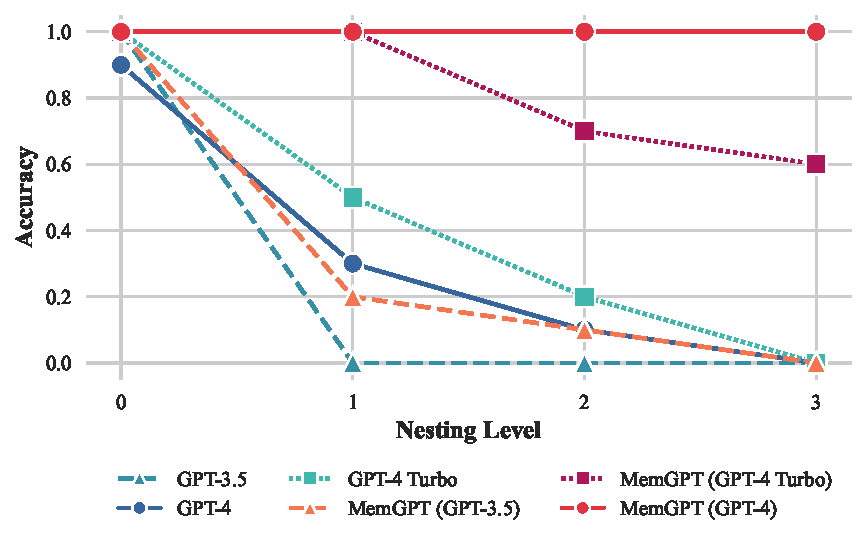
\includegraphics[width=0.45\textwidth]{images/nested_kv.pdf}
\end{center}
\caption{
\textbf{Nested KV retrieval task performance.}
\ours is the only approach that is able to consistently complete the nested KV task beyond 2 nesting levels.
While GPT-4 Turbo performs better as a baseline, \ours with GPT-4 Turbo performs worse than \ours with GPT-4. 
}
\label{fig:nested_kv_task_results}
\end{figure}

The document QA task is challenging for all methods due to the limitations of embedding-based similarity search.
We observe that the golden document for chosen question (as annotated by NaturalQuestions-Open) often appears outside of the first dozen retrieved results, if not even further.
The retriever performance translates directly to the fixed-context baseline results: GPT-4's accuracy is relatively low with few retrieved documents, and continues to improve as additional documents are added to the context window, as it correctly limits itself to answering questions based on information in retrieved documents. 
While \ours is theoretically not limited by sub-optimal retriever performance (even if the embedding-based ranking is noisy, as long as the full retriever ranking contains the gold document it can still be found with enough retriever calls via pagination), we observe that \ours will often stop paging through retriever results before exhausting the retriever database.


\begin{figure}[t!]
    \centering
\begin{center}
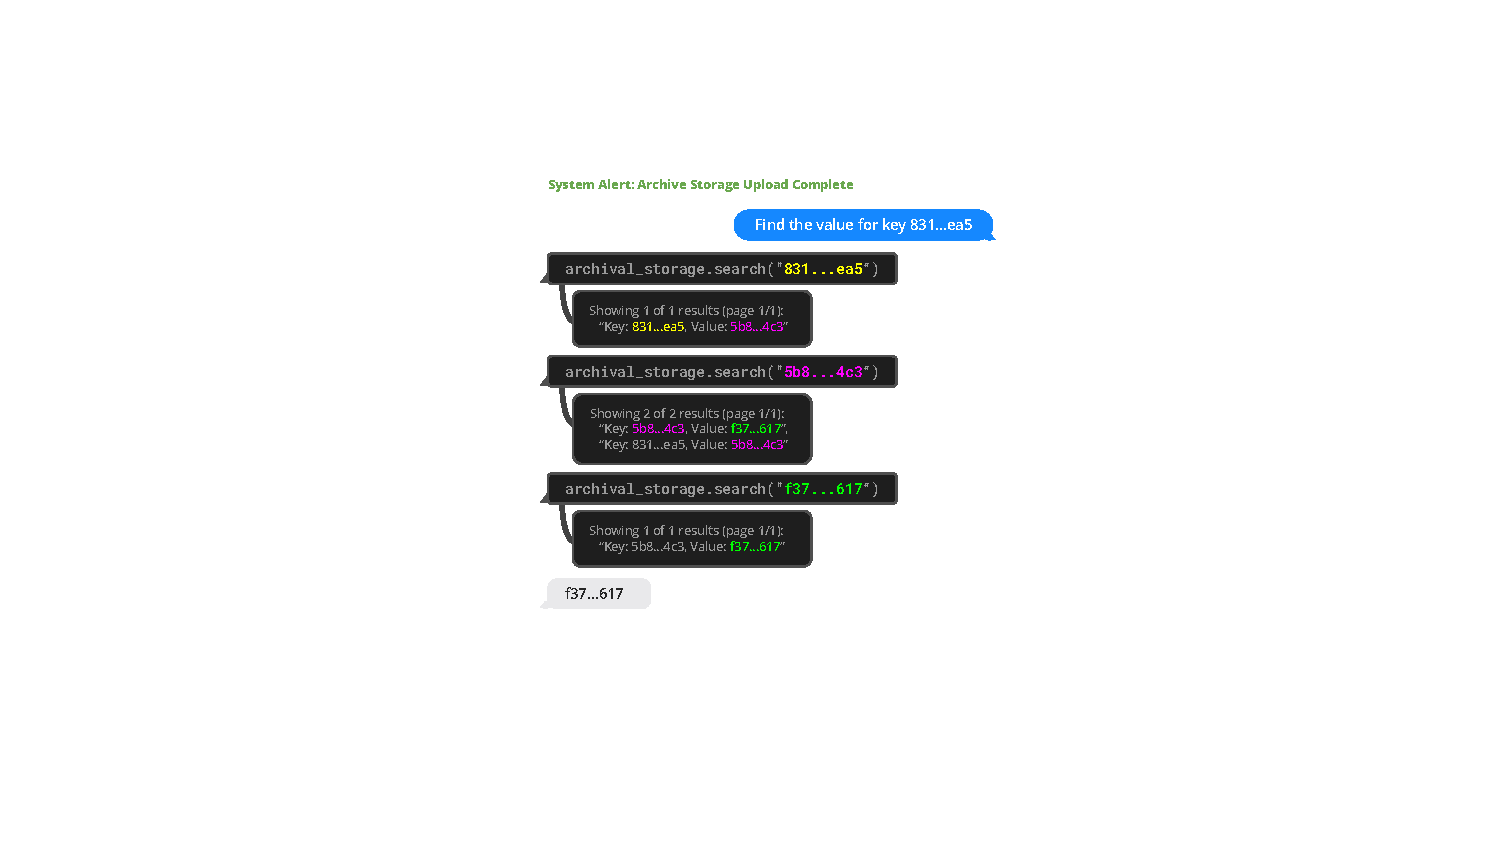
\includegraphics[width=0.45\textwidth]{images/memgpt_nested_kv_example.pdf}
\end{center}
    \caption{
An example of MemGPT (left) solving the nested KV task (UUIDs shortened for readability). In this particular example, the key-value pair has two nesting levels: \texttt{831..ea5} $\rightarrow$  \texttt{5b8..4c3} $\rightarrow$ \texttt{f37...617}.
The MemGPT agent returns the final answer when a query for the final value (\texttt{f37...617}) only returns one result, indicating that it is not also a key.
}
    \label{fig:example-nestedkv}
\end{figure}

To evaluate the fixed-context baselines against \ours past their default context lengths, we truncate the document segments returned by the retriever to fix the same number of documents into the available context.
As expected, document truncation reduces accuracy as documents shrink as the chance of the relevant snippet (in the gold document) being omitted grows, as shown in Figure \ref{fig:doc_qa_task_results}. 
\ours has significantly degraded performance using GPT-3.5, due to its limited function calling capabilities, and performs best using GPT-4.  







\subsubsection{Nested key-value retrieval (KV).}
We introduce a new task based on the synthetic Key-Value retrieval proposed in prior work \citep{liu2023lostinmiddle}. The goal of this task is to demonstrate how \ours can collate information from multiple data sources. In the original KV task, the authors generated a synthetic dataset of key-value pairs, where each key and value is a 128-bit UUID (universally unique identifier). The agent is then given a key, and asked to return the associated value for the key. We create a version of the KV task, \emph{nested KV retrieval}, where values themselves may be keys, thus requiring the agent to perform a multi-hop lookup.
In our setup, we fix the total number of UUIDs pairs to 140, corresponding to roughly 8k tokens (the context length of our GPT-4 baseline). We vary the total number of nesting levels from 0 (the initial key-value pair's value is not a key) to 4 (ie 4 total KV lookups are required to find the final value), and sample 30 different ordering configurations including both the initial key position and nesting key positions. 

While GPT-3.5 and GPT-4 have good performance on the original KV tasks, both struggle in the nested KV task. GPT-3.5 is unable to complete the nested variant of the task and has an immediate dropoff in performance, hitting 0 percent accuracy at 1 nesting level (we observe that its primary failure mode is to simply returns the original value). GPT-4 and GPT-4 Turbo are better than GPT-3.5, but also suffer from a similar dropoff, and hit 0 percent accuracy by 3 nesting levels. \ours with GPT-4 on the other hand is unaffected with the number of nesting levels and is able to perform the nested lookup by accessing the key-value pairs stored in main context repeatedly via function queries. \ours with GPT-4 Turbo and GPT-3.5 also have better performance than the corresponding baseline models, but still begin to drop off in performance at 2 nesting levels as a result of failing to perform enough lookups. 
\ours performance on the nested KV task demonstrates its ability to combine multiple queries to perform multi-hop lookups. 












